% Chapter 4

\chapter{SYSTEM DESIGN} % All Chapter headings in ALL CAPS

\section{SYSTEM ARCHITECTURE}

\tab In this project we propose a system which is designed to learn the image manipulation features and identify the authenticity of the given image. In this architecture the tampered images undergo a certain type of analysis and then it is fed into the neural network for further feature extraction and classification. The training dataset which contains the forged images are analysed for differences in the quality level which might occur due to the editing the image has undergone and resaving it. These comparisons in difference in quality levels within an image is done through the error level analysis and the output of this phase will be given to the CNN.

\tab Each convolutional layer is followed by a normalization process called batch normalization which will increase the accuracy of the CNN model.To give the accurate result the last layer in the classification layer of the neural network uses the softmax activation function which gives the highest activation level. The overall CNN architecture uses RMSprop optimizer which will help the model in converging faster.This will be used to identify the spliced images.
\tab For the detection of copy move forged images a block matching system is used.Where the image is split into blocks and some similarity functions are used to extract if they contain identical regions in the image which will ultimately prove that the image is tampered.
\newpage
\begin{figure}[htp]
\centering
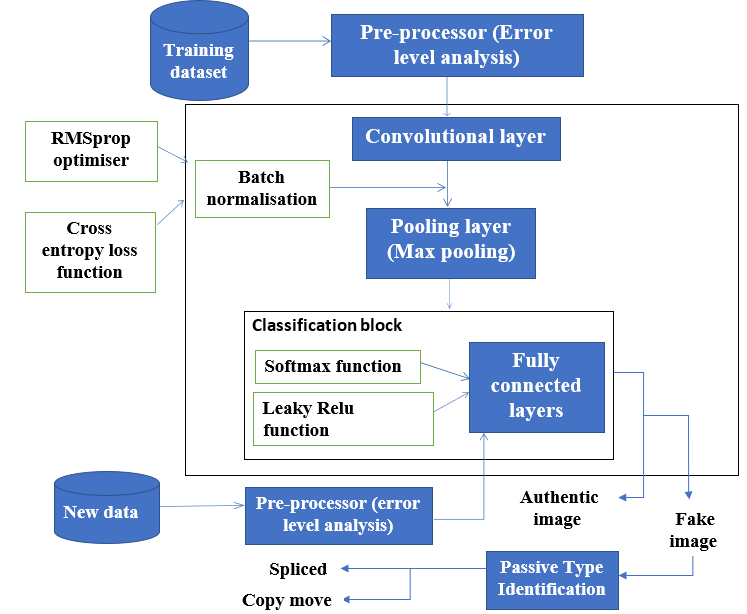
\includegraphics[scale=0.5,width=17cm]{Figures/ARC.PNG}
\caption{System Architecture}
\label{fig:universe}
\end{figure}
\newpage

\section{CLASS DIAGRAM}
The class diagram of the entire Recommendation system is showninfigure 4.3. This diagram depicts the functions of various modules in the system clearly. It also shows the interaction between the modules of the system thereby providing a clear idea for implementation.

\begin{figure}[h!]
\centering
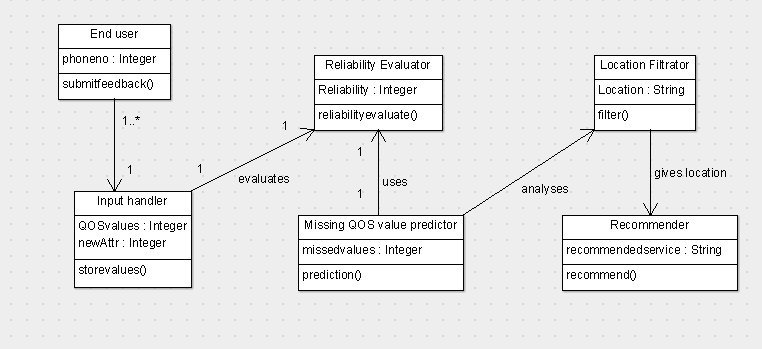
\includegraphics[scale=0.7]{overallcla}
\caption{Class Diagram}
\label{fig:universe}
\end{figure}

\section{MODULE DESIGN}
\subsection{DATA PREPROCESSING }
Images are preprocessed by performing error level analysis to focus on the detection of JPEG compression artifacts instead of feature extraction.JPEG uses a lossy image compression. Each re-encoding process (new saving) performed on the image leads to further loss of quality. The JPEG algorithm is based on a 8x8 pixel grid. Each 8x8 square grid is thereby treated and compressed separately. If the image is untouched, then all these 8x8 squares will show the same error level potential.  
 
\subsection{TRAINING THE CNN}
The CNN includes two layers one is feature extraction layer, the input of each neuron is connected to the local receptive fields of the previous layer, and extracts the local feature. Once the local features is extracted, the positional relationship between it and other features also will be determined. The other is feature map layer, each computing layer of the network is composed of a plurality of feature map. Every feature map is a plane, the weight of the neurons in the plane are equal.We consider the RMSProp optimizer  to train our model.The ReLU activation function is applied to each value in the feature maps of every convolutional layer. 
\subsubsection{RMSPROP OPTIMISER}
The RMSprop optimizer is similar to the gradient descent algorithm with momentum. The RMSprop optimizer restricts the oscillations in the vertical direction. Therefore, we can increase our learning rate and our algorithm could take larger steps in the horizontal direction converging faster.
\subsubsection{CROSS ENTROPT LOSS FUNCTION}
Cross entropy measures the divergence between two probability distribution, if the cross entropy is large, which means that the difference between two distribution is large, while if the cross entropy is small, which means that two distribution is similar to each other.When the difference between predicted value and actual value is large, the learning speed, i.e., convergence speed, is fast, otherwise, the difference is small, the learning speed is small.  

\subsection{CLASSIFICATION BLOCK}
This block contains layers of the CNN which accepts input as vectors.
To give the accurate result the last layer in the classification
layer of the neural network uses the softmax activation function which gives the highest activation level.The CNN model extracts the feature and classifies the pre-processed forged image to detect whether the given image is forged or not.

\subsection{PASSIVE TYPE DETECTION}
Passive image authentication is a class of authentication techniques that uses the received image itself only for assessing its authenticity or integrity, without any side information (signature or watermark) of the original image from the sender.
\begin{itemize}
    \item Splicing - It is a method of tampering images by combining two sources to produce a new image which retains the majority of one image for detail. 
    \item Copy-move - A copy move attack is commonly used to conceal parts of an image or to remove unwanted portions in an image. A portion from the picture is copied and pasted over any unwanted portion in the same image.
    \end{itemize}
    

\section{COMPLEXITY ANALYSIS}
\subsection{Complexity of the project}
\begin{itemize}
    \item  The complexity of the project lies in determining the passive type of forgery the image has undergone  rather than just determining if the image is only forged or not.The neural network is used to detect the spliced images.
    \item The accuracy of the neural network also affects the efficiency of the output. Hence efficient loss function and optimiser with the appropiate parameters needs to be chosen. 
    \item Certain additional hints need to be added to the images in order to efficiently detect the tampered regions in the images.Error level Analysis is used for this purpose.This anlaysis is made to all images irrespective of their formats and error potential.  
    \item Determining the identical regions in a copy move image is done by the extraction of similar properties between those regions for which efficient similarity functions has to be used. 
    \item The identification of copy move image is done without any comparison with the original image but rather the input image itself which makes it a tedious task to implement.
\end{itemize}